\documentclass[onecolumn, draftclsnofoot, 10pt, compsoc]{IEEEtran}
\usepackage{graphicx}
\usepackage{url}
\usepackage{setspace}
\usepackage{geometry}
\usepackage{listings}
\usepackage{caption}

\geometry{textheight=9.5in, textwidth=7in}

% 1. Fill in these details
\def \CapstoneTeamName{			Team 41}
\def \CapstoneTeamNumber{		41}
\def \GroupName{				30k CS Avionics}
\def \GroupMemberOne{			Joshua Novak}
\def \GroupMemberTwo{			Allison Sladek}
\def \GroupMemberThree{			Levi Willmeth}
\def \CapstoneProjectName{		30K Rocket Spaceport America}
\def \CapstoneSponsorCompany{	Oregon State University}
\def \CapstoneSponsorPerson{	Dr. Nancy Squires}

% 2. Uncomment the appropriate line below so that the document type works
\def \DocType{		%Problem Statement
					%Requirements Document
 					%Technology Review
 					%Preliminary Design Document
					Winter Progress Report
				}
			
\newcommand{\NameSigPair}[1]{
	\par
	\makebox[2.75in][r]{#1} \hfill
	\makebox[3.25in]{\makebox[2.25in]{\hrulefill} \hfill \makebox[.75in]{\hrulefill}}
	\par\vspace{-12pt}
	\textit{
		\tiny\noindent \makebox[2.75in]{} \hfill
		\makebox[3.25in]{\makebox[2.25in][r]{Signature} \hfill \makebox[.75in][r]{Date}}
	}
}
% 3. If the document is not to be signed, uncomment the RENEWcommand below
%\renewcommand{\NameSigPair}[1]{#1}
% \renewcommand{\thesubsubsection}{\thesection.\alph{subsubsection}}

%%%%%%%%%%%%%%%%%%%%%%%%%%%%%%%%%%%%%%%
\begin{document}
\begin{titlepage}
    \pagenumbering{gobble}
    \begin{singlespace}
    	%\includegraphics[height=4cm]{coe_v_spot1}
        \hfill 
        % 4. If you have a logo, use this includegraphics command to put it on the coversheet.
        %\includegraphics[height=4cm]{CompanyLogo}   
        \par\vspace{.2in}
        \centering
        \scshape{
            \huge CS Capstone \DocType \par
            {\large\today}\par
            \vspace{.5in}
            \textbf{\Huge\CapstoneProjectName}\par
            \vfill
%             {\large Prepared for}\par
%             \Huge \CapstoneSponsorCompany\par
%             \vspace{5pt}
%             {\Large\NameSigPair{\CapstoneSponsorPerson}\par}
            {\large Prepared by }\par
%            	\GroupName\par
            % 5. comment out the line below this one if you do not wish to name your team
%             \CapstoneTeamName\par
            \vspace{5pt}
            {\Large
                \NameSigPair{\GroupMemberOne}\par
                \NameSigPair{\GroupMemberTwo}\par
                \NameSigPair{\GroupMemberThree}\par
            }
            \vspace{20pt}
        }
    \end{singlespace}
    
    \section*{Revision History}
    \begin{tabular*}{1\linewidth}{@{\extracolsep{\fill}}|c|c|c|c|}
      \hline
      Name & Date & Reason For Changes & Version\\
      \hline
      Levi Willmeth, Joshua Novak, Allison Sladek&2/9/18&Initial document draft&0.1\\
      \hline
    \end{tabular*}
	\\
    
    \begin{abstract}
    Winter project report covering the current design, progress, technical challenges and solutions for the computer science portions of the Oregon State University (OSU) American Institute of Aeronautics and Astronautics (AIAA) team's entry in the Spaceport America Cup 30k competition during the summer of 2018.  The competition involves designing, building, and launching a student-made rocket to 30,000 feet.
	\end{abstract}
\end{titlepage}
\newpage

\pagenumbering{arabic}

\tableofcontents
% 7. uncomment this (if applicable). Consider adding a page break.
%\listoffigures
%\listoftables

%===============================================================================
%Start Problem Statement w/o Metrics
\newpage
\section{Project Overview}
This computer science (CS) capstone project includes providing technical and software support to the Oregon State University (OSU) American Institute of Aeronautics and Astronautics (AIAA) team's entry for the Spaceport America Cup 30k competition in the summer of 2018.  The competition involves designing, building, and launching a student-made rocket to 30,000 feet.

Our goals are to learn new skills and gain experience while working together as a team to build a rocket, and to also score well during the Spaceport America Cup competition.  The scoring metric rewards teams that provide avionics to control the rocket, receive live telemetry on the ground during the flight, and can visualize the results of an onboard scientific payload after the flight.  Our task will be to write the software necessary to accomplish those goals.

The AIAA team includes several sub teams that will all need to work together.  In particular, we need to work with the electrical and computer engineering (ECE) students who are responsible for developing the avionics hardware and telemetry radio systems.  The ECE subteam is ultimately responsible for those systems, but we will provide support and write the necessary avionics software to be used during flight.

Our subteam will focus on designing a ground system capable of collecting and viewing flight data, and programs to control flight avionics for the rocket and scientific payload.

We recognize that it is also important to support the overall team, because at the competition we will all succeed or fail together.  As such, we need to attend regular team meetings and generally understand the challenges faced by our teammates, as well as our own.

%===============================================================================

\section{Designs and Solutions}

%-------------------------------------------------------------------------------

\subsection{Ground Station}
Section by Levi Willmeth
\subsubsection{Overview}
The project requires building a ground station program to receive, parse, store, and serve all of the data recorded during the rocket's flight.  This information will be made available to users over a web page served over local WiFi.

\begin{center}
	\includegraphics[width=0.5\textwidth]{images/parser_diagram.eps}
    \label{gs-diagram}
    \captionof{figure}{Flow of information through the ground station.}
\end{center}

\subsubsection{Current Progress}
We built a ground station which is enclosed inside a hard travel box.  The box protects the delicate electrical components from the harsh environment of the New Mexico desert, where the final competition will be held.  Inside the box we assembled four Raspberry Pi Zero computers, each with it's own USB sound card.  Each Zero is powered from a USB port on a central Raspberry Pi 3B computer, which hosts a MariaDB database, ad-hoc WiFi network, and NodeJS server.

A 22,000 mAh rechargeable battery allows the entire ground station to operate for up to 12 hours on a single charge. We also purchased a spare battery and backups for each of the Pi computers and ground station components because there's a hard-learned saying about redundancy in critical systems:  'two is one, one is none.'

\begin{center}
	\includegraphics[width=0.5\textwidth]{images/ground_station_closeup.eps}
    \label{gs_closeup}
    \captionof{figure}{The current ground station without protective padding in place.}
\end{center}

A LCD in the ground station shows useful at-a-glance information such as the status of each parser, and the last known location of both the rocket and payload.  This information is queried directly from the database every two seconds, to reduce load while maintaining accuracy.

\begin{center}
	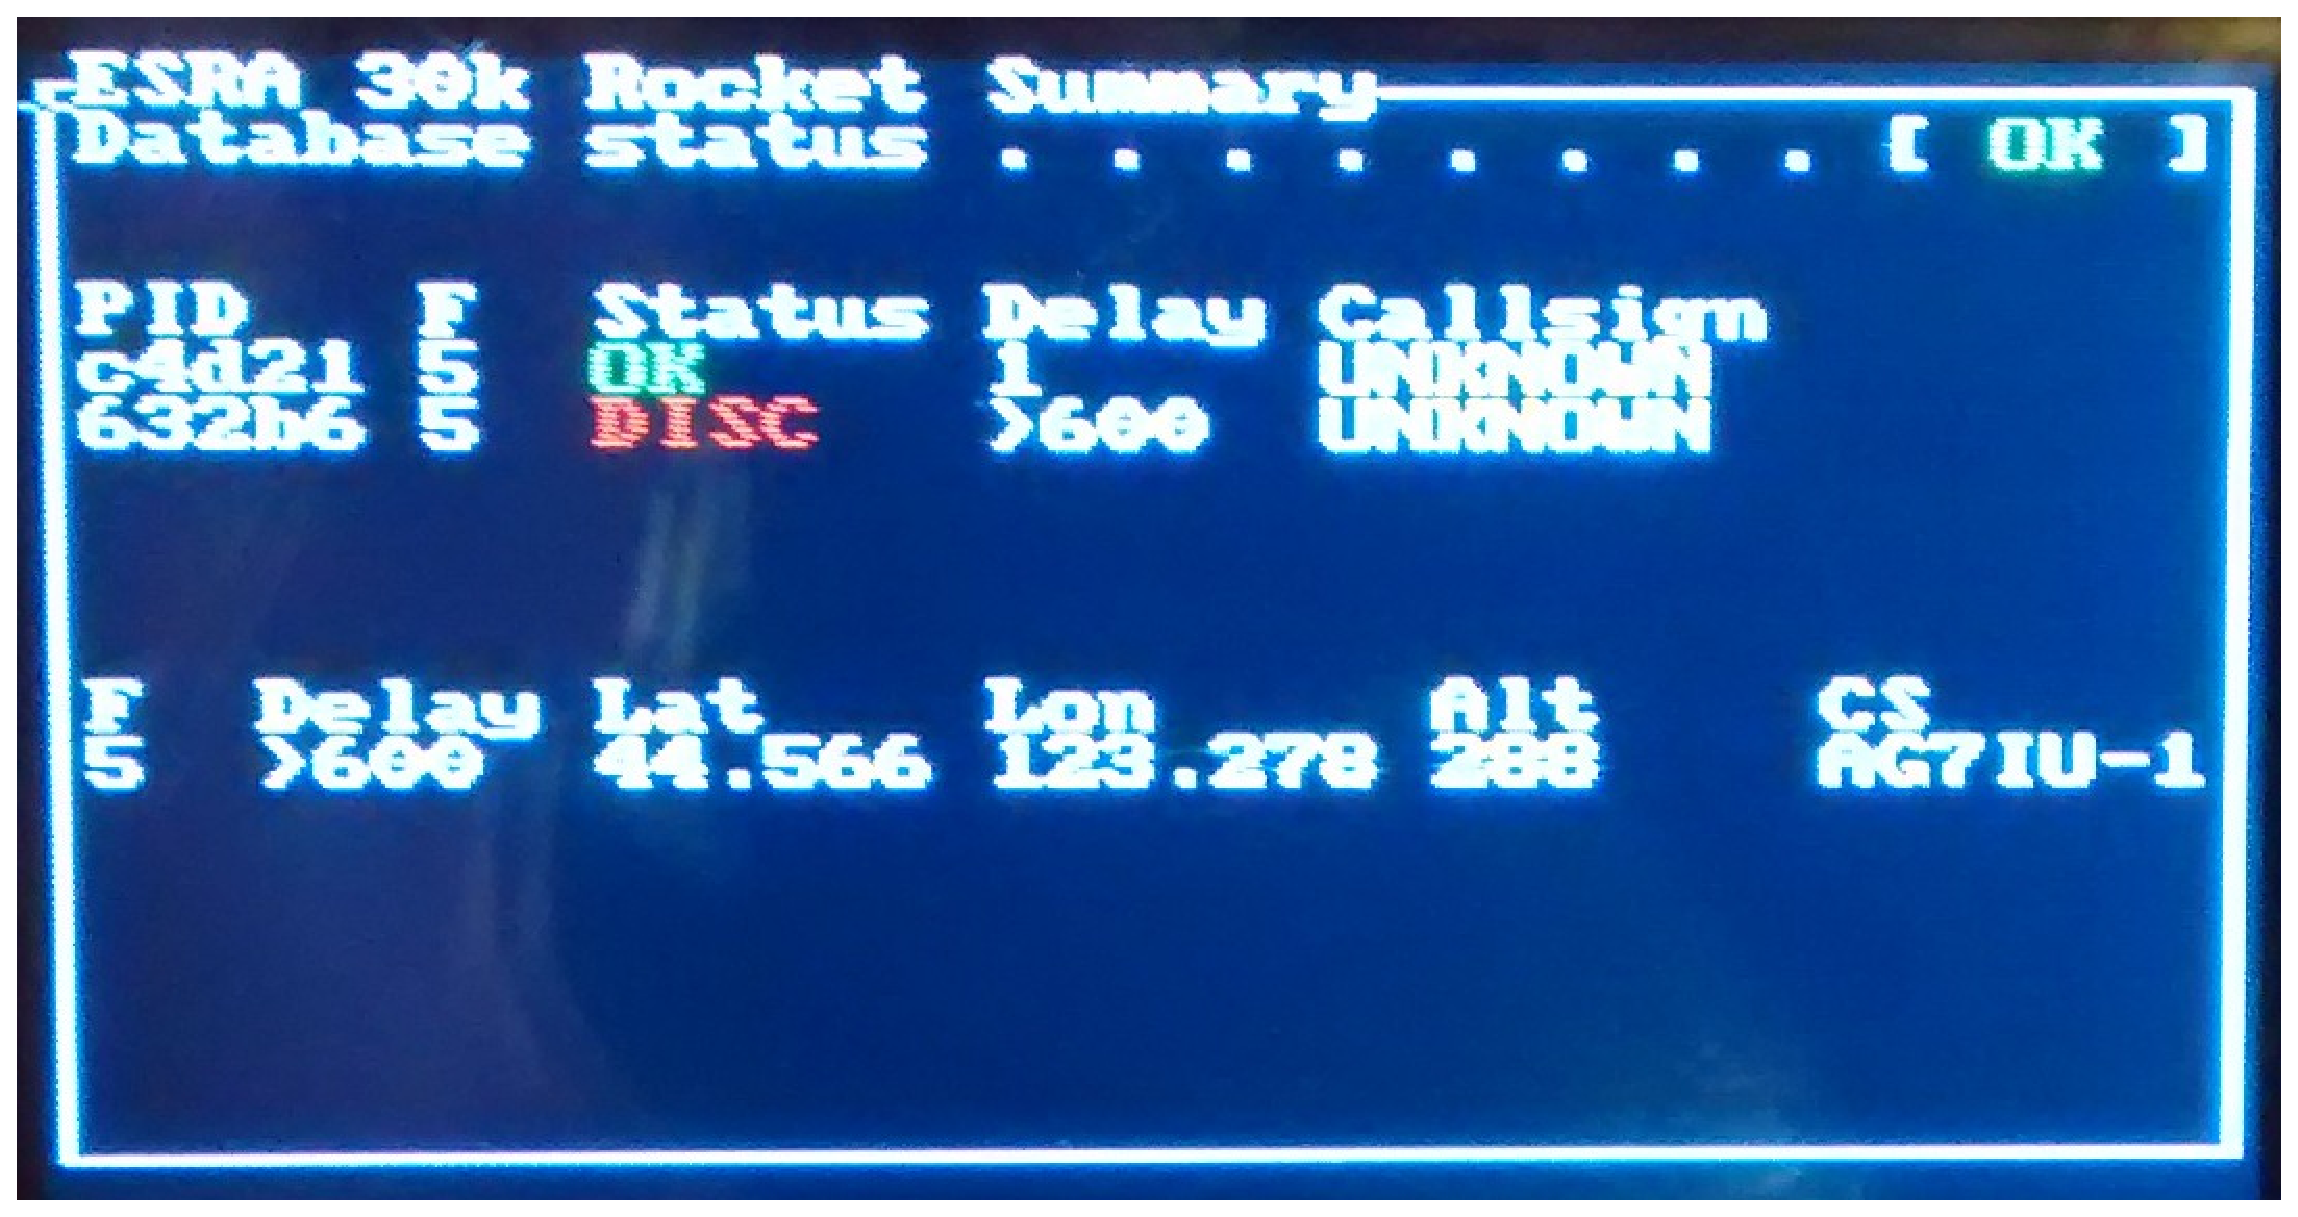
\includegraphics[width=.5\textwidth]{images/monitor.eps}
    \label{gs-monitor}
    \captionof{figure}{LCD in the ground station showing parser status and last location from the database.}
\end{center}

\subsubsection{Remaining Tasks}
The physical assembly has been a challenge for us.  We don't have the manufacturing tools and knowledge to reliably secure the components in way that is also visually appealing.  We assembled the ground station using plastic sheets and foam padding that are not ideal.

To solve this problem, we enlisted the help of a junior mechanical engineering student on the team, who is 3d printing a more visually impressive system to hold the computers and battery in place.  This is an good example of learning to work with our ESRA team members from different backgrounds, to create a better component than we could manufacture on our own.

The current ground station is effective and meets our goals, but we would like to make it look better.

%-------------------------------------------------------------------------------

\subsection{Networking}
Section by Allison Sladek

\subsubsection{Overview}
The Raspberry Pi 3B computer in the ground station will serve a local Wi-Fi network that nearby people can join to interact with our system. 
Each of the Raspberry Pi Zero computers will be networked to the main Pi 3B computer using USB OTG, which allows them to be powered and networked over a single USB cable.  
We will be able to ssh into the Pi 3B or Pi Zeros using this Wi-Fi network. 
This system should allow our teammates to connect to our web interface to view incoming flight data during the launches as well as any stored data from previous launches after it has been uploaded. 

\subsubsection{Current Progress}
The main Raspberry Pi 3B has been configured to connect to any known Wi-Fi networks, or broadcast its own if there is none available. 
This was done by editing configuration files on the Pi. This network has been sufficient for testing purposes, but a stress test during one of our weekly meetings revealed some issues. 
Out of our group of about 25 people, about half of the room had some connectivity issues with our website. 

The USB on-the-go connection was fairly straightforward to configure, and doesn’t currently have any known issues.
The Raspberry Pi 3B is able to communicate with the Raspberry Pi zeros.


\subsubsection{Remaining Tasks}
The stress test results reveal the next area of progress for our network. 
We may need to add additional hardware, or change something about our hosting software to provide service to our whole team at launch day. 
During the test, our graphs made very frequent queries to the database to check for updated data points.
This may also be part of the reason for some of our outages, but overall more testing is needed.

%-------------------------------------------------------------------------------

\subsection{Graphs}
Section by Joshua Novak
\subsubsection{Overview}

Our goal is to create a readable display for the telemetry data received during and after flights. It should be able to display certain data within ten seconds of it being sent from the rocket, and should also be able to display data that has been uploaded to the database after a launch.
\subsubsection{Current Progress}

The Raspberry Pi 3B currently serves a web interface that users can connect to on mobile devices. This interface queries the database to receive new data at regular intervals, updating as new information is added to the database. Currently there are three plots, the altitude vs time plot, the vertical velocity vs time plot, and the gps coordinate plot. The altitude vs time plot is setup to receive input from up to six sources that correspond with a single flight ID, and plots the altitude of the rocket as recorded by that source vs the time it was recorded. The vertical velocity graph is similar, but instead displays the change in altitude, thus the specification of it being the vertical velocity. This is used instead of recorded velocity because we do not receive any recorded velocity mid-flight. Finally, the GPS coordinate map can plot the location of the rocket recorded by any source on a map. We use a saved map from google images for testing, and will likely do the same for the final map.

\subsubsection{Remaining Tasks}

We are planning to implement other graphs as well, such as acceleration, heading, and temperature. These have not yet been implemented because we will not be receiving that data mid-flight, so these graphs were put at a lower priority. We also plan to enhance the visuals of the map to be more readable, marking recorded locations with colored buttons and having the colors vary by time or altitude, making it easier to tell the flight path of the rocket at a glance. This has a higher priority since it will be useful for ensuring that people can clearly see the trajectory of the rocket during a flight.

Recent additions to the graphing have mostly been restricted to implementing graphs from multiple sources. This has not yet been used in an end to end test, but should be able to display graphs from all sources that have the same flight id. The different sources will show up as separate graphs. 

%-------------------------------------------------------------------------------

\subsection{Data Parser}
Section by Levi Willmeth
\subsubsection{Overview}
The parsing program takes an audio source for live telemetry data from a hand held radio, or a CSV file of raw sensor values created by the onboard avionics computers.  The program should validate audio telemetry data using a checksum, and by comparing expected fields.  It will then write the information into a database on the same network.

\subsubsection{Current Progress}
The current data parser successfully runs simultaneously on four raspberry pi zeros in the ground station.  Each zero has a USB sound card and can process an audio signal from either BeelineGPS telemetry unit on the rocket, as well as parse the first-generation sensor files created by our beta payload avionics.  The parsed data is immediately saved in the MariaDB database on the main raspberry pi 3, also in the ground station.

We used a test file created by the ECE subteam which uses progressively weaker signals, to compare the performance of our parser against several other similar commercial products.  Our parser was able to decode 30/50 of the signals, compared to most commercial solutions decoding 30-31 and the absolute best commercial solution reportedly decoding 42/50.  We believe the difference comes from the quality of our inexpensive sound card vs a desktop PC dedicated sound card. We will continue to try to improve our performance, but are generally satisfied with our current results.

\subsubsection{Remaining Tasks}
The CSV files created by our beta payload avionics only include the MPU6050 and BMP180 sensors, so these files will change as the payload avionics evolve and the ECE subteam finalizes the sensor components.

As a stretch goal, we also want to be able to parse and store signals from the TeleMega telemtry unit, which includes many more data fields than the BeelineGPS.  These signals should be very similar to the actual payload files.  Instead of an audio signal, the TeleMega outputs serial data over USB, which should be readable from our parser program.

%-------------------------------------------------------------------------------

\subsection{Database}
Section by Levi Willmeth

\subsubsection{Overview}
The database is served by a Raspberry Pi 3B computer inside the ground station case.  The database collects and stores all data recorded during the flight, and relates records inserted at different times and from different sources by using a combination of primary and foreign keys. This will allow our web server to select records based on a given flight, or range of time, even though flight records are stored across several tables.

\subsubsection{Current Progress}
The database was one of the first components built and has not needed any recent updates.  There are some tables like Logs that are not currently being used, but we expect that the flight avionics systems will eventually utilize those as necessary.

Currently the BeelineGPS, Flights, Parser\_Status, and Payload\_Avionics tables are being actively used by our system, and are meeting our needs. We have been able to write all of the queries needed to insert telemetry and flight avionics data, as well as select that data to use in the display client.

\begin{center}
	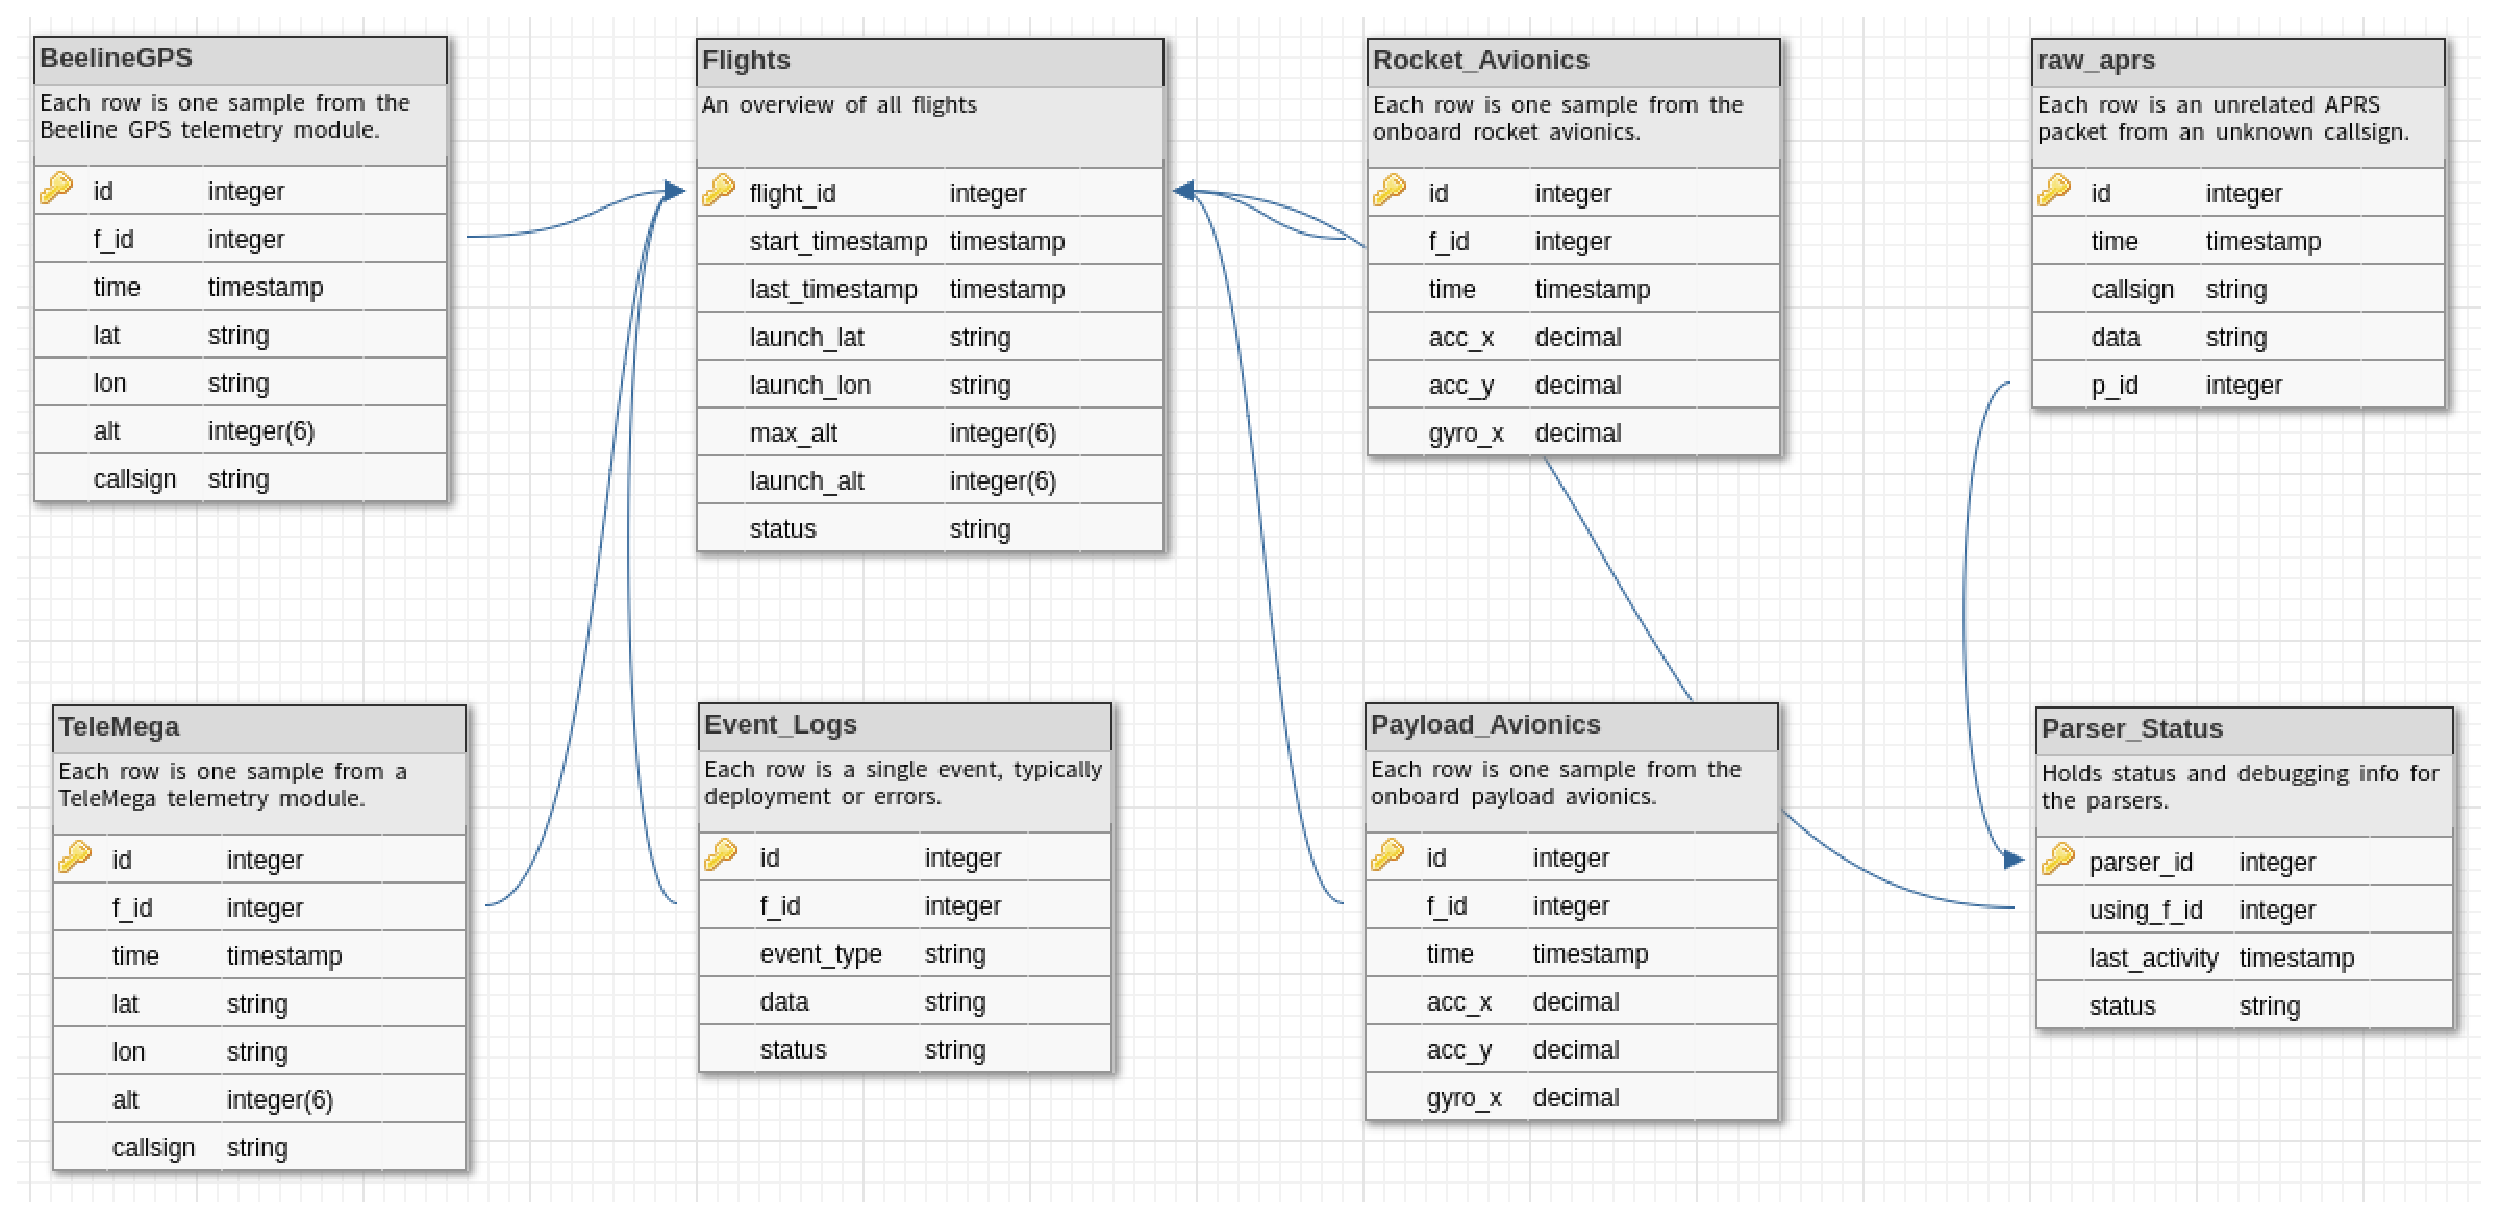
\includegraphics[width=.8\textwidth]{images/database_schema_v102.eps}
    \label{database-schema}
    \captionof{figure}{Current state of our database schema.}
\end{center}

\subsubsection{Remaining Tasks}
As the project continues we may find a need to update the database schema or make changes, but for now we consider the database to be finished.

%-------------------------------------------------------------------------------
\subsection{Sensor Avionics}
Section by Joshua Novak
\subsubsection{Overview}
For sensor avionics, the primary goal is to retrieve values from the different sensors installed on the rocket and format them into floats to be processed by the other avionics programs on the Raspberry Pi's. The sensors are connected to over an I2C bus, and will have some modifactions made to them by the ECE's as part of the requirements for their capstone.

\subsubsection{Current Progress}
Curently we are able to read from all of the different sensors that we know will be used aside from two, the new accelerometer which will double as a magnetometer and the real time clock. We have had some issues with different sensors sharing I2C addresses, as the accelerometers and the real time clock all use the same address, though the accelerometers can also be set to a second address. Our solution has been to send a signal to the different sensors to have them change address, then receive values from each of them after they have been swapped to a unique address. Another major issue has been the speed limitations on the bus. Without making use of the I2C buffer, the amount of time it takes to get a new reading from a sensor is significant, taking the roughly 5 khz that the sensors can run at down to a 100 hz loop if all three accelerometers are accessed. However, if we were to switch to the buffer, there would be a larger delay to retrieve values (though we would get more). Another issue would be with implementing our address switching alongside use of the buffer, meaning we would have to either only utilize one acceleromteter (which would be far from ideal considering that gives us a single point of failure for all avionics code and significant readings, as they are based on the accelerometer) or increase the time it takes to retrieve all of the different values to a much greater degree. We decided that getting values that were recent was more important than getting more values, and therefore will not be using the buffer. Because of this we will get less values, but they will be more recent. This has led to us switching to using Python for our code, since the speed gains of using C are not significant as roughly 90 percent of runtime is spent waiting for the bus. Python has gains for us in other areas, such as having a much larger variety of libraries written for it, and being easier to debug and write tests for. Finally, a new idea of recording values to a database instead of a CSV will be easier and faster to implement in Python than in C, which may have significant speed gains as we will not need to convert values to strings, which takes up a signifcant portion of runtime.

\subsubsection{Remaining Tasks}
A number of checks need to be implemented in the sensor avionics. Firstly, two additional sensors (our new accelerometer and our real time clock) have not yet been implemented, as we have only recently received the clock and have not yet received the new accelerometer. Also, checks to insure values are within bounds have not been implemented into the sensor avionics code. Most sensors have a maximum range for their values, and therefore it should be easy to detect when a value of is out bounds, since the space of in bounds values is small compared to out of bounds values. An integrity check will be inserted into the code for each sensor, checking that the values are in range for what the sensor would record, and also are not out of bounds for what we would expect during our launches (such as discarding an altimeter reading of over 100k feet). 
%-------------------------------------------------------------------------------
\subsection{Rocket Avionics}
Section by Allison Sladek
\subsubsection{Overview}
The primary goals of the rocket avionics are to read and record values from the rocket sensors at a reasonable rate, ensure those stored values are recoverable after launch, and detect and record the moment of apogee. 
Many of these functions are similar to the functions of the payload avionics, so we may reuse code from each section for the other. 
The sensors have to be checked and recorded as quickly as is reasonable with the resources available.
More frequent samples will give more detailed data of the launch and allow better testing and analysis for post-launch. 
The values of the sensor data will be to be stored on the pi and made available after recovery of the rocket, or else no data will be revered from the launch, hindering our efforts of testing the rocket.
Apogee detection is very important to the success of the rocket. It normally triggers separation and parachute ejection, and without sensing it correctly, the rocket may deploy its parachute at the wrong time, or not at all. 

\subsubsection{Current Progress}
At the beginning of the project, it was stated that our rocket avionics would detect and trigger separation of the rocket, at apogee.  
Some time over winter, it was decided that the flight computer would not be connected to the separation charges.  
This decision was made by the ECE subteam without communicating with us.  As such, it will be impossible for us to trigger separation.
Instead, we will continue with our plan to detect apogee.  Instead of triggering separation, we will write a line to the log file.  That's as close as we can get to meeting our original goal of triggering separation.

As much of the functions of the payload and rocket avionics overlap, there will likely be reused solutions between the two. 
As such, while there hasn’t been much headway on the reading/storing of sensor data for the rocket avionics in particular, there has been a lot of work done for this solution in the payload avionics programming.

The primary area of progress for the rocket avionics is the function originally planned to be unique to the rocket avionics: apogee. 
A common method for apogee detection is using a magnetometer, which can help determine apogee based on the earth’s magnetic field. 
The rocket does include a magnetometer, but the proximity of the sensor to metals makes this method unreliable. 
Instead, we will be using a combination of the 3-axis accelerometer and the altimeter. 
The moment of apogee is defined by the point at the apex of the flight in which the rocket has a total acceleration of zero and the altitude changes from increasing to decreasing. 
Between these two sensors, we can test both of these statements at any given point to determine the moment of apogee. 


\subsubsection{Remaining Tasks}
Apogee detection has yet to be implemented. 
We plan to use data primarily from the 3-axis gyroscope and the altimeter with some statistical methods to reduce erroneous data, as well as some failsafes to ensure that apogee is detected. 
This would be mission critical if we still planned on triggering separation, because deploying too early or too late means the rocket will be in the wrong position when the parachute deploys, if it deploys at all. 
This would drastically reduce our chances of a successful recovery of the rocket as a whole. 
We still plan on writing our code as if it was carrying out a critical task, so the failsafes will be in place to ensure that we don’t skip the separation event.
The logic for our apogee detection will look something like this:

\begin{minipage}{\linewidth}
  \begin{lstlisting}[frame=single]
  If total acceleration <= somewhat close to zero g:
      Start a countdown timer.
      If apogee hasnt been logged when it goes off, log apogee event.

  If total acceleration <= very close to zero g:
      Start a much shorter countdown timer.
      If apogee hasnt been logged when it goes off, log apogee event.

  If altitude begins to decrease:
      Log apogee event.

  If total acceleration hits one of our thresholds and then starts to increase again:
      Apogee has occurred. If it hasnt been logged, log it now.
  \end{lstlisting}
\end{minipage}

The exact threshold values for "somewhat close" and "very close" to zero will need to be determined by consulting some of the mechanical engineering teams and our mentors. 

%-------------------------------------------------------------------------------

\subsection{Payload Avionics}
Section by Levi Willmeth

\subsubsection{Overview}
The Payload Avionics have two primary goals: use a propeller to push the payload towards the ground at the correct rate in order to neutralize gravity, and record data from onboard sensors to an SD card for later analysis.

The payload will be ejected from the body of the rocket at apogee, and attempt to create a zero gravity environment for 10-12 seconds during descent.  An array of sensors on the payload will rapidly measure the kinematics experienced by the payload.  A closed PID loop will use the latest acceleration values to calculate and control a pair of motors.  One motor will pull the payload downwards using a 10" propeller.  The second motor will spin a small weight in the opposite direction, to stabilize the rotation of the payload.  In this way, we hope to accelerate downwards at the same rate as gravity, to simulate stable spin and zero acceleration for 10-12 seconds.

Simultaneously, the payload will log sensor values onto an SD card in order to later analyze the performance of the payload and experiment.

\subsubsection{Current Progress}
Currently, the payload avionics are able to read from the current batch of sensors, which include three MPU6050's for acceleration and rotation, a BMP180 for altitude and temperature, a PCF8523 for accurate timestamps, and a magnetometer for bearing.  The ECE subteam is selecting the list of flight sensors and has yet to finalize these components.  It has been a challenge to not have control over the sensors used because it is difficult to make progress without knowing the components we will be using.  We have adapted by asking them which sensors they are likely to use, purchasing our own set of those sensors, and informing them that we cannot guarantee to support hardware changes made after winter term.  That seems like a reasonable solution to us, and they seem to be responding positively as well.

The current version of the payload avionics software reads all of these sensors, uses a PID loop to calculate a motor speed based on the current acceleration, motor speed, and the time since last motor update.  It uses the output of that calculation to drive the propeller's brushless motor via an attached ESC.

Finally, the avionics logs the values used during this loop to a text file in CSV format.  Because there are several sensors, and each sensor has several values, the current version of the avionics software creates a CSV file which has around 18 values per line, and is generated at a rate of 107 Hz, or lines per second.

Currently, all sensor values are written on every line.  As we add additional sensors and begin optimizing for performance, we will probably begin writing certain sensor values more often than others.  For example, the altimeter is our slowest sensor and has an accuracy of +/- several meters.  Instead of logging the altitude at 20 Hz, we could reduce it to ~5 Hz and significantly increase the rate of the rest of our loop.  This should improve our primary goal of achieving zero acceleration by increasing the rate of our motor speed calculations.

Another potential improvement we are exploring is using a database on the payload instead of writing to a CSV file.  This may allow us to insert values faster, or increase our accuracy by writing floats instead of truncated strings for most of our sensor values.  We are currently working to implement a test case to compare runtimes between CSV and database insertions.

\subsubsection{Remaining Tasks}
We need to implement the second motor, which spins a small weight in the opposite direction to provide counter torque.  The motor and PID classes that we wrote should allow us to do this relatively easily.

We also need to test the rather arbitrary PID values that we selected.  These values are based on the physical properties of our system, and cannot be accurately calculated mathematically.  They depend on the reaction time of the motors, the amount of torque each motor generates, and the amount of thrust the propeller generates at different RPM.

We also need to write more unit tests.  This is something that we have fallen behind on.  We have been prototyping various changes so quickly that writing tests hasn't made much sense until we knew what we would stick with.  At this point we have a pretty good idea about what works, and should begin writing better tests.


%-------------------------------------------------------------------------------

\section{Support the AIAA team as a whole}
\subsubsection{Overview}
Another goal for this project is to support the entire team, not just the computer science subteam.  To do our part, we will attend regular team meetings and try to understand the problems and challenges faced by the other subteams.  If we see an opportunity to help another subteam with something, we will do our best to do so.  We will also attend the majority of team building and training exercises, as well as all practice rocket launches.

\subsubsection{Current Progress}
As of the middle of Winter term, each of us have attended almost every team meeting.  On the rare occasion someone is unable to make it to a meeting, they have always been in contact with the other subteam members to let them know.

\subsubsection{Remaining Tasks}
This task requires upkeep, so we will keep going to meetings.

%===============================================================================

\end{document}
